\documentclass{beamer}
\usepackage[T1]{fontenc}

\usepackage{polski}
\usepackage[utf8]{inputenc}
\usepackage[polish]{babel}
%
% Choose how your presentation looks.
%
% For more themes, color themes and font themes, see:
% http://deic.uab.es/~iblanes/beamer_gallery/index_by_theme.html
%
\mode<presentation>
{
	\usetheme{Warsaw}      % or try Darmstadt, Madrid, Warsaw, ...
	\usecolortheme{crane} % or try albatross, beaver, crane, ...
	\usefonttheme{default}  % or try serif, structurebold, ...
	\setbeamertemplate{headline}{}
	\setbeamertemplate{caption}[numbered]
} 

\title[Praca magisterska]{Rekomendacje artykułów opisujących produkty w serwisach e-commerce}
\author{Łukasz Dragan}
\institute{Informatyka spec. Metody sztucznej inteligencji, MiNI PW}
\date{31.10.2017}

\begin{document}
	
	\begin{frame}
		\titlepage
	\end{frame}
	
	\begin{frame}{Plan prezentacji}
	  \tableofcontents
	\end{frame}
	
	\section{Cel pracy}
		\begin{frame}{Cel pracy}
			Czy metody semantycznej analizy tekstu mogą być alternatywą dla~dotychczas uzywanej przez~\emph{Allegro} metody generowania rekomendacji artykułów tekstowych?
		\end{frame}
		\begin{frame}{Dlaczego?}
			wypisać swoją motywację
		\end{frame}
	\section{Opis problemu}
	
	\begin{frame}{pracuj.pl}
		\begin{figure}
			\centering
			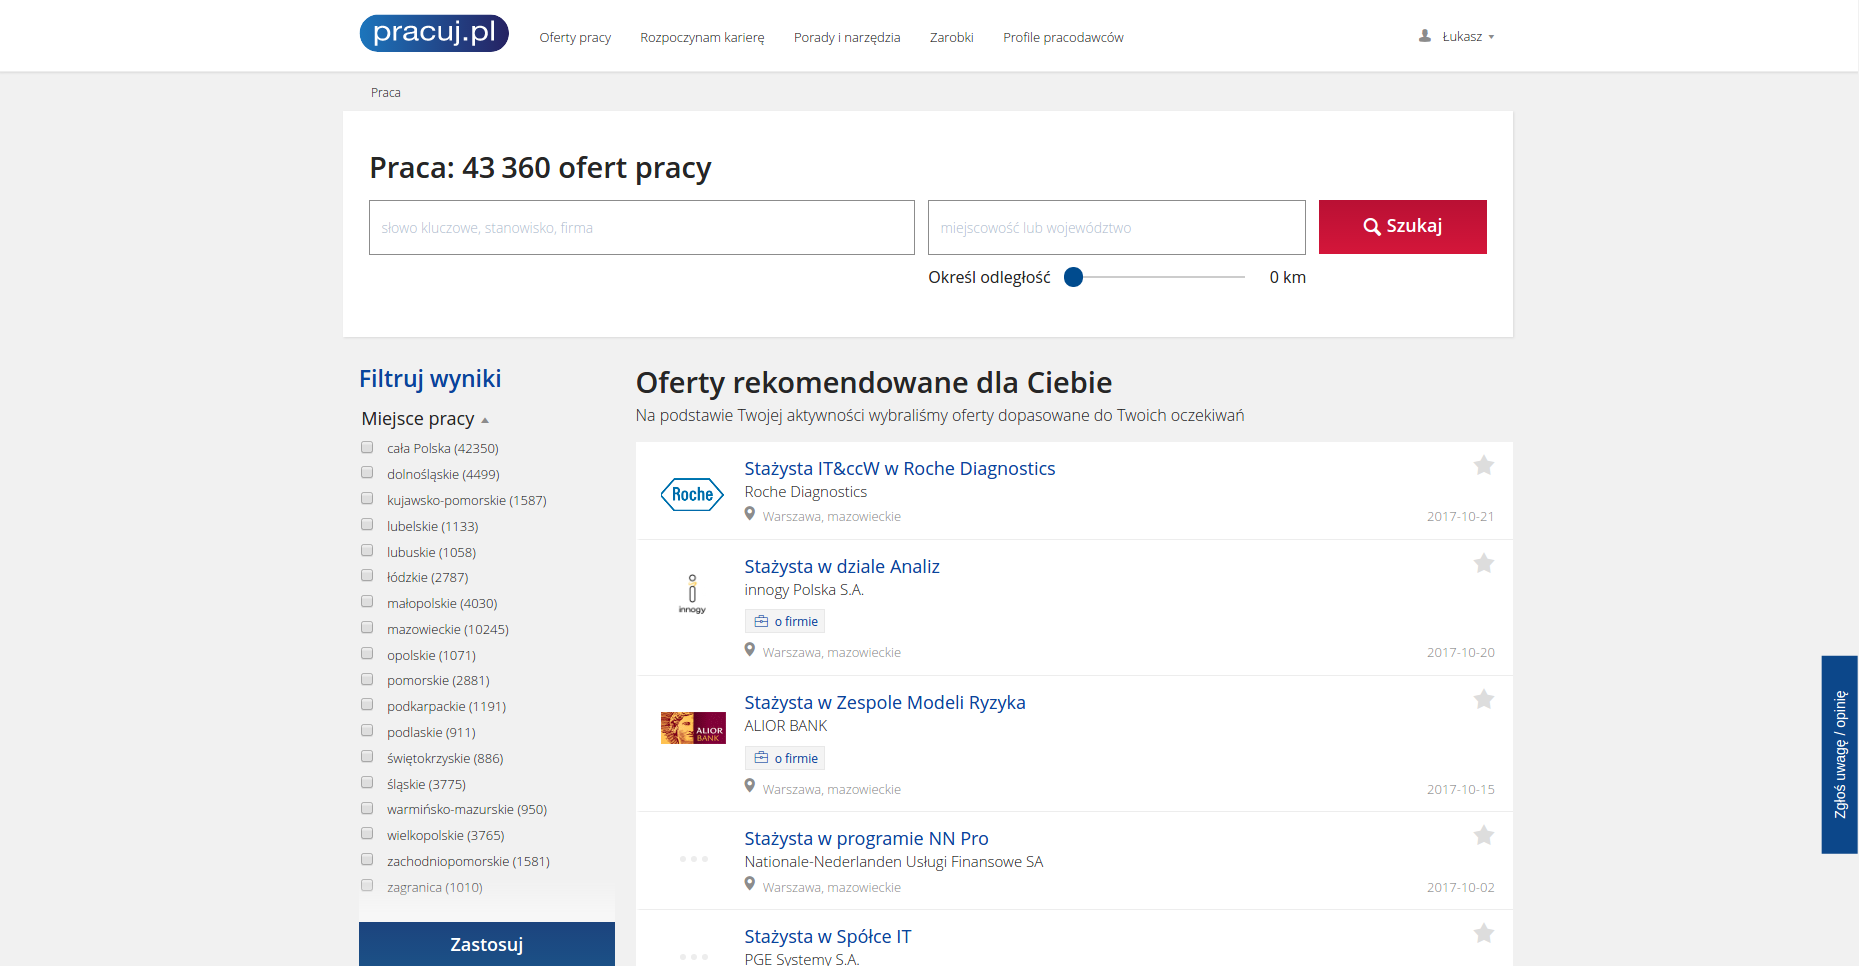
\includegraphics[width=1\textwidth]{img/pracuj.png}
		\end{figure}
	\end{frame}
	
	\begin{frame}{filmweb.pl}
		\begin{figure}
			\centering
			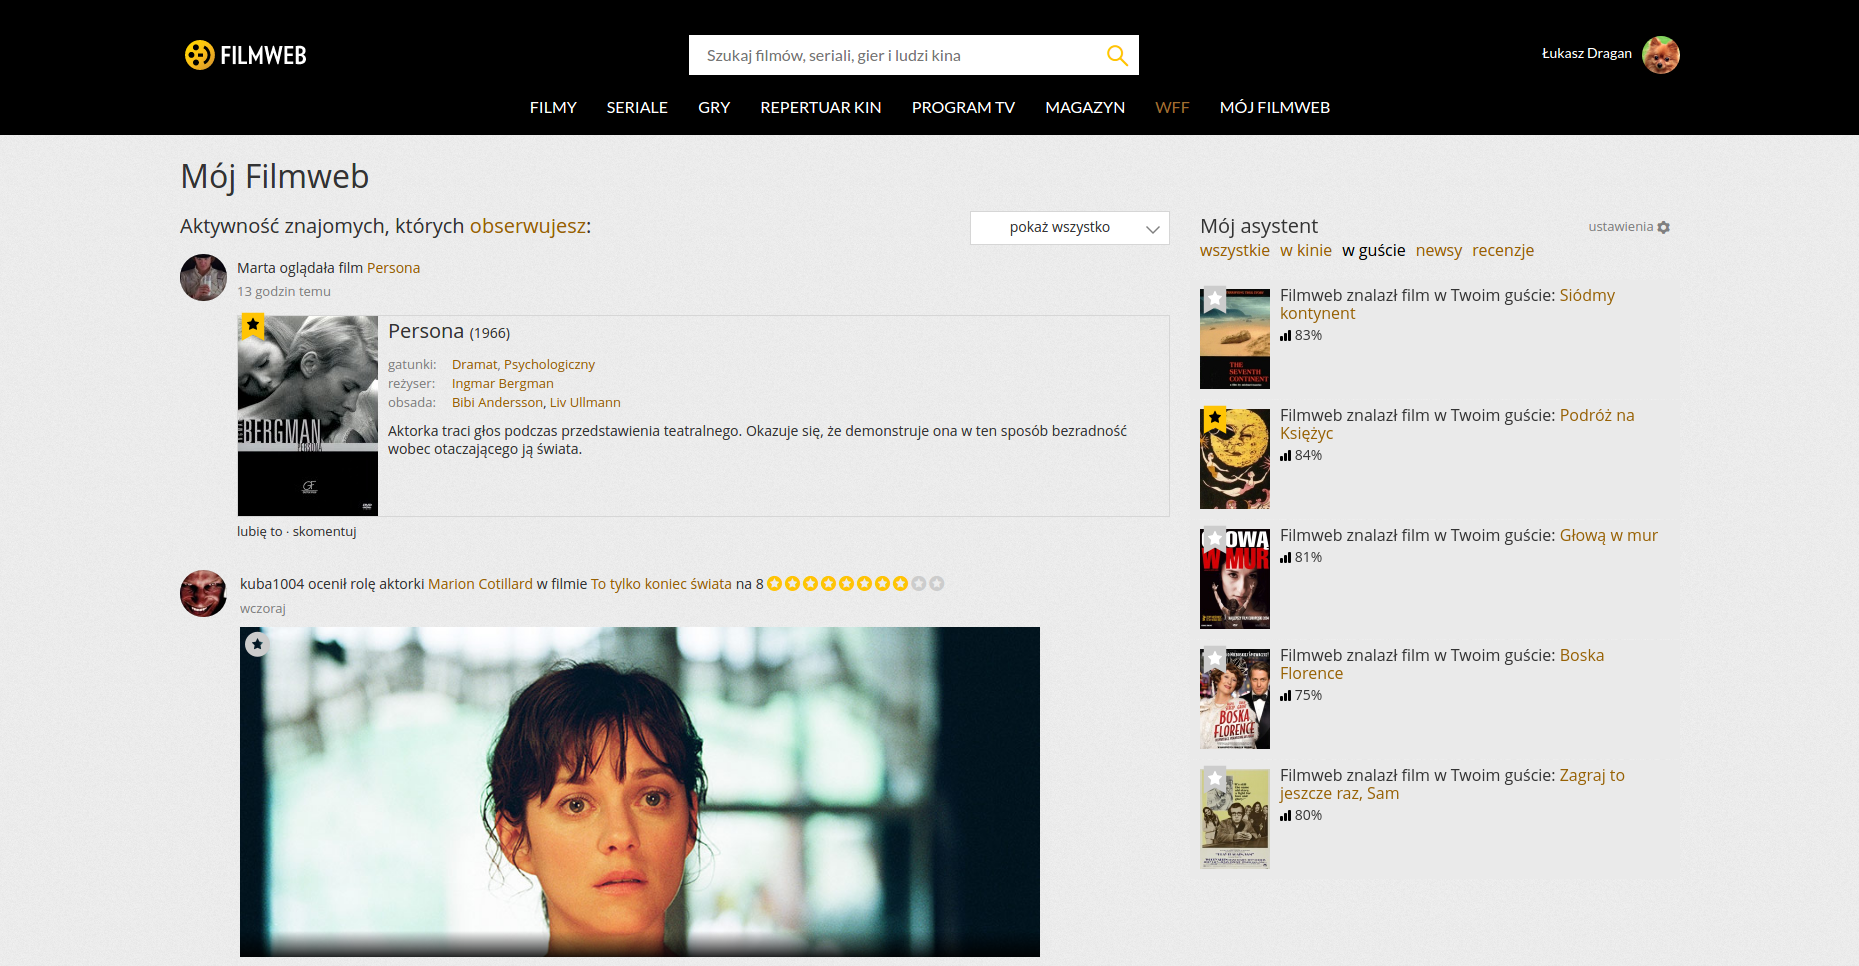
\includegraphics[width=1\textwidth]{img/filmweb.png}
		\end{figure}
	\end{frame}
	
	\begin{frame}{allegro.pl}
		\begin{figure}
			\centering
			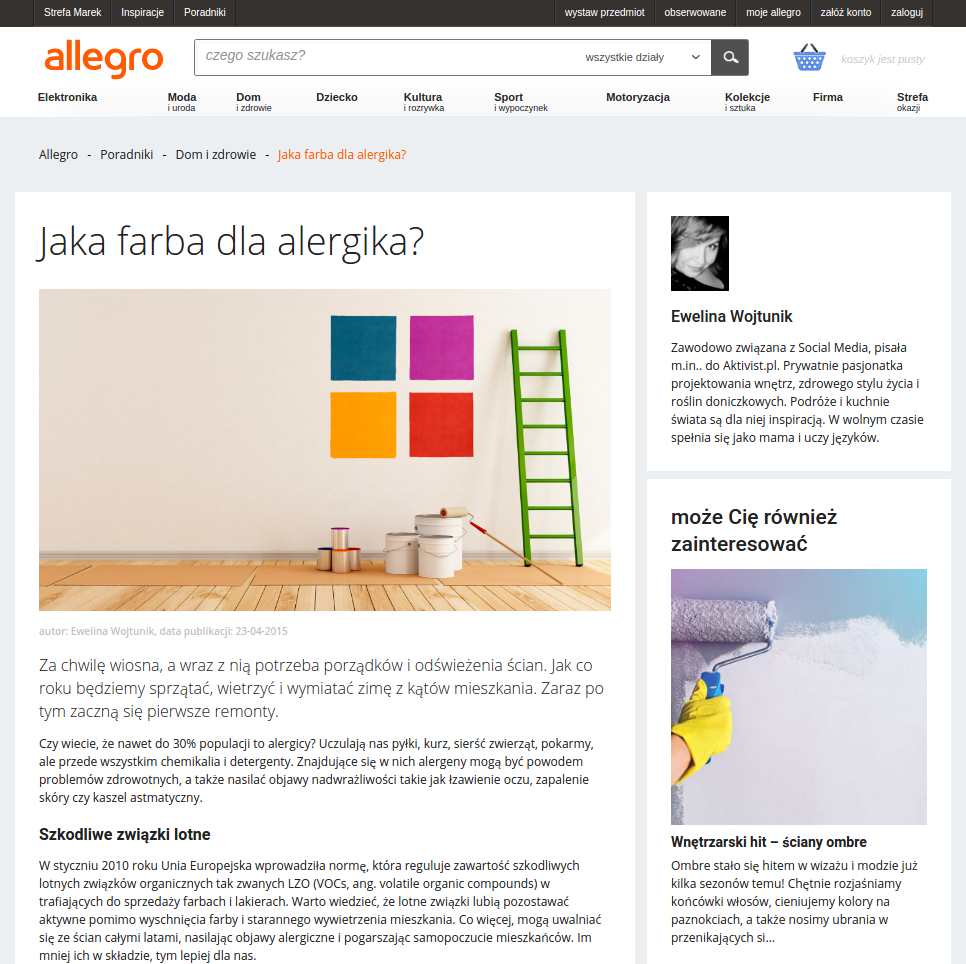
\includegraphics[width=1\textwidth]{img/screen_allegro.png}
		\end{figure}
	\end{frame}
	
	\begin{frame}{allegro.pl cd}
		\begin{figure}
			\centering
			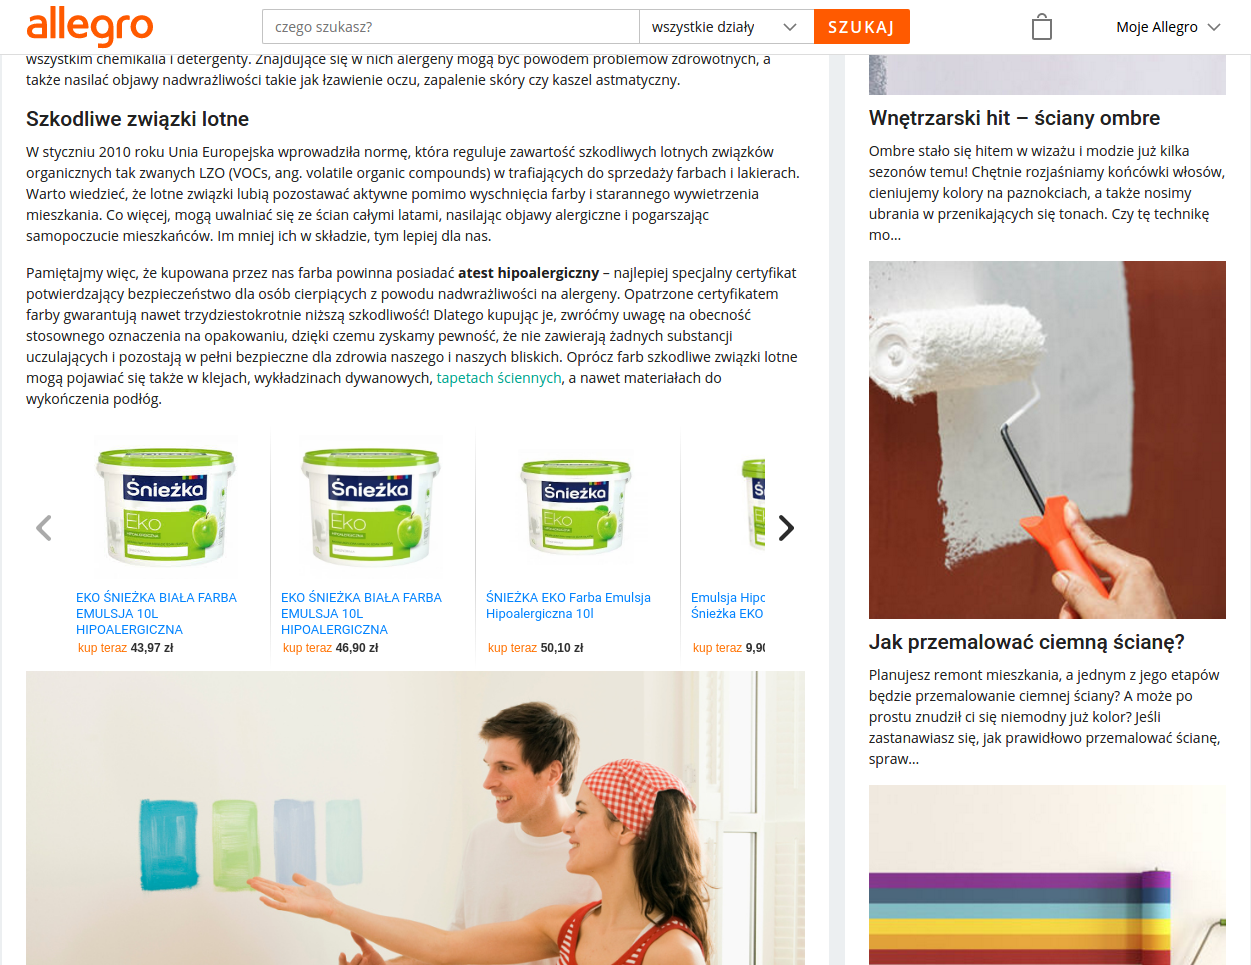
\includegraphics[width=1\textwidth]{img/screen_allegro_2.png}
		\end{figure}
	\end{frame}
	
	\section{Systemy rekomendacji}
	\begin{frame}{Elasticsearch}
		\begin{figure}
			\centering
			
\includegraphics[width=0.5\textwidth]{img/elastic-logo.png}
		\end{figure}
		,,Elasticsearch is a distributed, JSON-based search and analytics engine designed for horizontal scalability, maximum reliability, and easy management.''
	\end{frame}

	\begin{frame}{Systemy rekomenadacji}
		%TODO
		W ujęciu ogólnym systemy wyszukiwania mają na~celu sugerowanie tego, co użytkownik chciałby otrzymać. Natomiast systemy rekomendacji mają sugerować przedmioty potrzebne użytkownikowi nawet, jeżeli potrzeby te nie~zostały bezpośrednio wyrażone.
	\end{frame}
	
	\begin{frame}{Systemy rekomenadacji}
		\begin{figure}
			\centering
			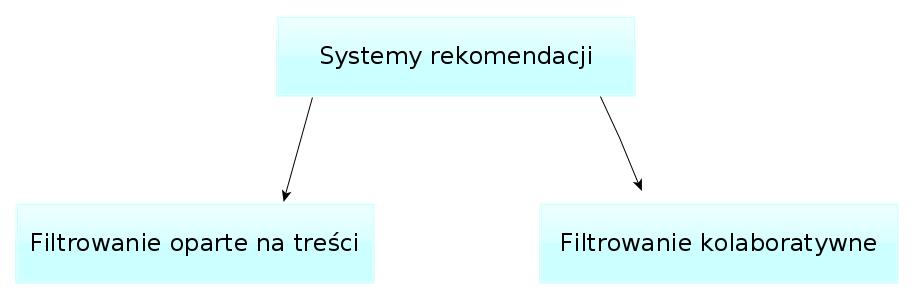
\includegraphics[width=1\textwidth]{img/recommender.png}
		\end{figure}
	\end{frame}
	\section{Techniki przetwarzania języka naturalnego}
	\begin{frame}{Zarys podejścia}
		\begin{figure}
			\centering
			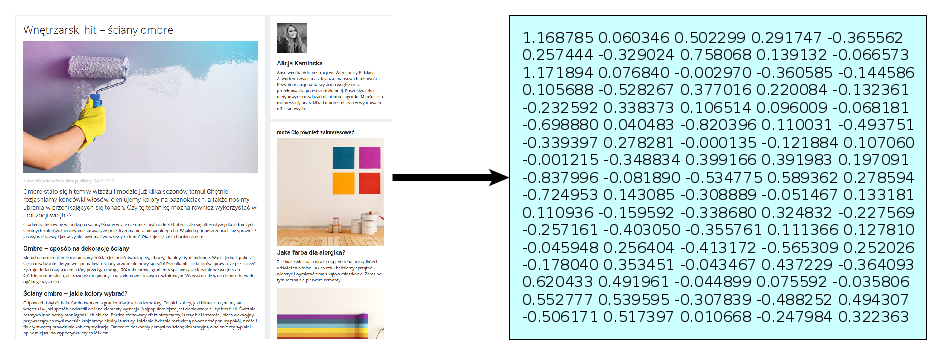
\includegraphics[width=0.85\textwidth]{img/approach_outline.png}
		\end{figure}
		\pause
		\begin{figure}
			\centering
			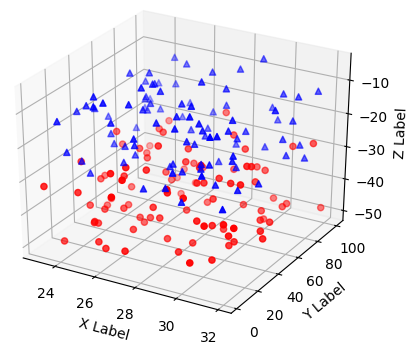
\includegraphics[width=0.45\textwidth]{img/scatter3d_demo.png}
		\end{figure}
	\end{frame}
	\subsection{Bag-of-words}
	\begin{frame}{Bag-of-words}
		\begin{figure}
			\centering
			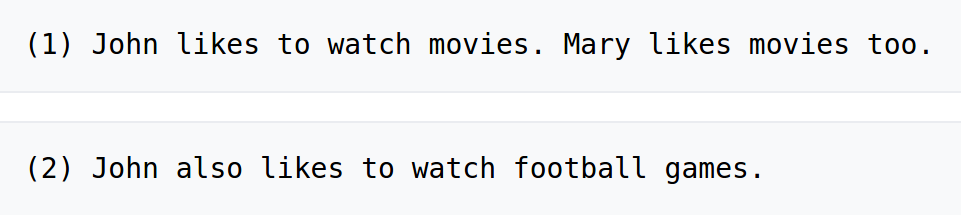
\includegraphics[width=0.75\textwidth]{img/bow_sents.png}
		\end{figure}
		\pause
		\begin{figure}
			\centering
			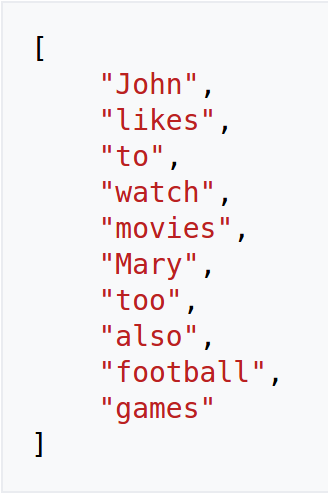
\includegraphics[width=0.25\textwidth]{img/bow_dict.png}
		\end{figure}
		\pause
		\begin{figure}
			\centering
			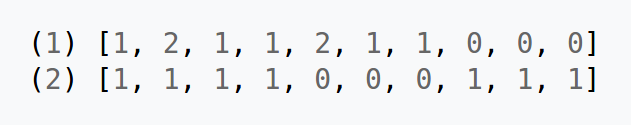
\includegraphics[width=0.5\textwidth]{img/bow_repr.png}
		\end{figure}
	\end{frame}
	\begin{frame}{Bag-of-words}
		Zalety:
		\begin{itemize}
			\item prostota \pause
		\end{itemize}
		Wady:
		\begin{itemize}
			\item duża wymiarowość wektorów \pause
			\item traktowanie każdego słowa z~jednakową wagą
		\end{itemize}
	\end{frame}
	\subsection{TF-IDF}
	\begin{frame}{TF – term frequency, IDF – inverse document frequency}
		Wartość \textit{TF-IDF} słowa $w_i$ w dokumencie $d_j$:
		\begin{equation}
		\label{eq:tf-idf}
		tfidf_{ij} = tf_{ij} * idf_i,\ tf_{ij} = \frac{n_{ij}}{\sum\limits_{k}n_{kj}},\ idf_i = log\frac{|D|}{|{d:w_i \in d}|}
		\end{equation}
		\begin{itemize}
			\item $tf_{ij}$: liczba wystąpień słowa $w_i$ w~dokumencie $d_j$ podzielona przez~liczbę słów dokumentu $d_j$,
			\item $idf_i$: liczba dokumentów w~korpusie podzielona przez~liczbę dokumentów zawierających przynajmniej jedno wystąpienie słowa $w_i$.
		\end{itemize}
	\end{frame}
	\begin{frame}{TF-IDF}
		Przykład analogiczny do bow
	\end{frame}
	\begin{frame}{TF-IDF}
		Zalety:
		\begin{itemize}
			\item nadal prostota \pause
			\item ważenie słów w~zależności od~częstości występowania \pause
		\end{itemize}
		Wady:
		\begin{itemize}
			\item nadal duża wymiarowość wektorów
		\end{itemize}
	\end{frame}
	\begin{frame}{Semantyka dystrybucyjna}
		Distributional hypothesis --- ,,słowa występujące w~tym samym kontekście niosą ze~sobą podobne znaczenie.''
		%Kolejne, bardziej zaawansowane, omawiane tu metody opierają się na~tzw. distributional hypothesis --- hipotezie zakładającej, że słowa występujące w~tym samym kontekście niosą ze~sobą podobne znaczenie. Sprzyja to zastosowaniu metod algebry liniowej jako narzędzia obliczeniowego oraz sposobu reprezentacji tekstu. Podstawowe podejście polega na~zgromadzeniu informacji o~rozkładzie słów w~dokumentach w~postaci wielowymiarowych wektorów, a~następnie wyodrębnieniu podobieństw pomiędzy~tymi wektorami, które świadczyłyby o~pewnych powiązaniach między reprezentowanymi słowami.
	\end{frame}
	\subsection{Modelowanie tematów}
	\begin{frame}{Modelowanie tematów}
		%Że jest to rodzaj redukcji wymiarowości
	\end{frame}
	\subsection{Latent semantic analysis}
	\subsection{Latent Dirichlet allocation}
	\subsection{Osadzanie słów w przestrzeni wektorowej}
	\begin{frame}{Word embeddings}
		\begin{itemize}
			\item Osadzanie słów w przestrzeni wektorowej
			\item Uczenie nienadzorowane
			\item Niska wymiarowość wektorów
			\item Reprezentacja słów wraz z~zależnościami pomiędzy nimi
		\end{itemize}
		\pause
		\begin{figure}
			\centering
			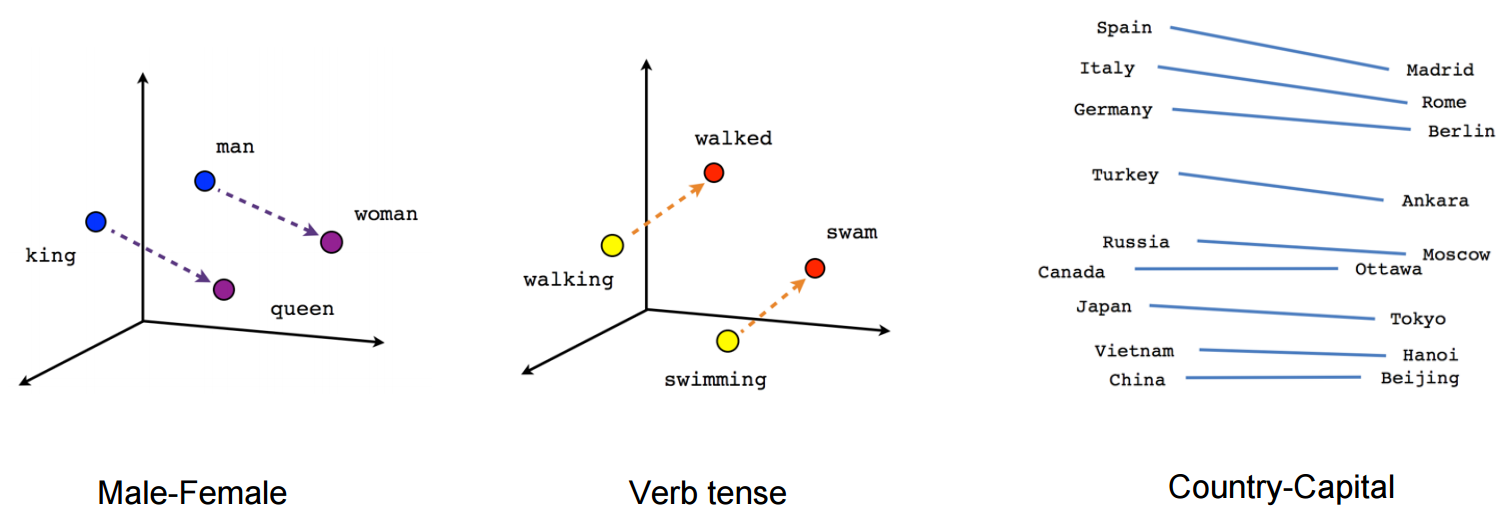
\includegraphics[width=1\textwidth]{img/linear-relationships.png}
		\end{figure}
		%https://www.tensorflow.org/images/linear-relationships.png
	\end{frame}
	% live demo z word2vec jeżeli starczy czasu
	\begin{frame}{Wektorowa postać dokumentu}
		
	\end{frame}
	
	\begin{frame}{Odległość między dokumentami}
		centroid, autorskie lda i wmd
		wmd dać przykładowy rysunek obama
	\end{frame}

	\begin{frame}{{Miary oceny wyszukiwania}}
		precision, recall, f-measure, ndcg
	\end{frame}	

	\begin{frame}{Analiza danych}
		\begin{itemize}
			\item 20000~artykułów tekstowych w~formacie \textit{JSON}
			\item język polski
			\item słowa specyficzne dla różnych branż
			% ,,hipertoniczny'', ,,autofocus''
			\item struktura artykułu:
			\begin{itemize}
				\item treść: tytuł, nagłówek, tekst
				\item metadane: id, kategoria, słowa kluczowe
			\end{itemize}
			% w pracy opisuję dokładne statystyki
		\end{itemize}
	\end{frame}
	\begin{frame}{Wstępne przetwarzanie danych}
		\begin{enumerate}
			\item Oczyszczanie tekstu ze znaczników \pause
			\item Usunięcie słów stopu
		\end{enumerate}
	\end{frame}
	\begin{frame}{Słowa stopu}
		a, aby, ach, acz, aczkolwiek, aj, albo, ale, ależ, ani, aż, bardziej, bardzo, bo, bowiem, by, byli, bynajmniej, być, był, była, było, były, będzie, będą, cali, cała, cały, ci, cię, ciebie, co, cokolwiek, coś, czasami, czasem, czemu, czy, czyli, daleko, dla, dlaczego, dlatego, do, dobrze, dokąd, dość, dużo, dwa, dwaj, dwie, dwoje, dziś, dzisiaj, gdy, gdyby, gdyż, gdzie, gdziekolwiek, gdzieś, go, i...
	\end{frame}
	\subsection{Wstępne przetwarzanie danych}
	\begin{frame}
		\begin{enumerate}
			\item Oczyszczanie tekstu ze znaczników
			\item Usunięcie słów stopu \pause
			\item Zamiana na małe litery \pause
			% większości duże litery na początku zdania przeszkadzają, ale czasem wyraz z dużej litery i z małej znaczą co innego - Włochy
			\item Tokenizacja i lematyzacja % morfologik.blogspot.com
		\end{enumerate}
	\end{frame}
	\begin{frame}{Preprocessing - przykład}
		\begin{figure}
			\centering
			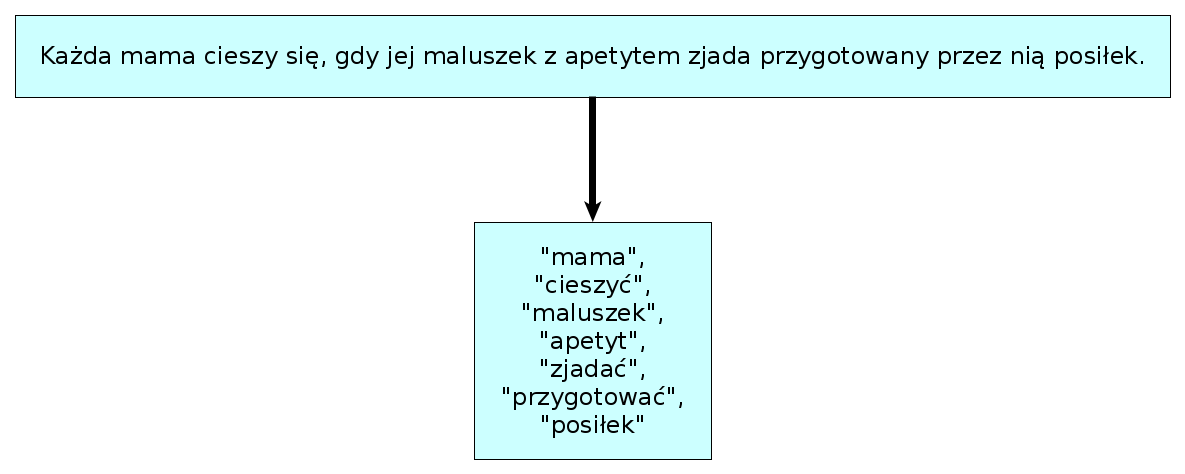
\includegraphics[width=1\textwidth]{img/lemmatisation.png}
		\end{figure}
	\end{frame}
	\section{Metody ewaluacji}
	\begin{frame}{Metody ewaluacji}
		\begin{enumerate}
			\item \textit{clicks} --- ocena na~podstawie historycznej aktywności użytkowników mierzona na~podstawie liczby kliknięć w~odnośniki.
			\item \textit{mut\_cat[\_ndcg]} --- relewantność wyszukanych artykułów liczona na~podstawie liczby wspólnych kategorii z~artykułem bazowym. Stosuję dwa warianty: średnia relewantność wyszukanych artykułów oraz~miara \textit{nDCG}.
			\item \textit{mut\_kw[\_ndcg]} --- relewantność wyszukanych artykułów liczona na~podstawie liczby wspólnych słów kluczowych z~artykułem bazowym. Również stosuję dwa warianty: średnia relewantność wyszukanych artykułów oraz~miara \textit{nDCG}.
			\item \textit{users} --- ocena na~podstawie eksperckiej oceny użytkowników. W~badaniu wykorzystałem 5~użytkowników operujących każdy na~tym samym zbiorze par testowych. Pary zostały wygenerowane (zgodnie z~wcześniejszym opisem metody) na~podstawie 50 artykułów bazowych wylosowanych spośród wszystkich artykułów udostępnionych mi przez~\textit{Allegro}.
		\end{enumerate}
	\end{frame}
	\section{Testy}
	\begin{frame}{LSI w zależności od liczby tematów}
		\begin{figure}[H]
			\centering
			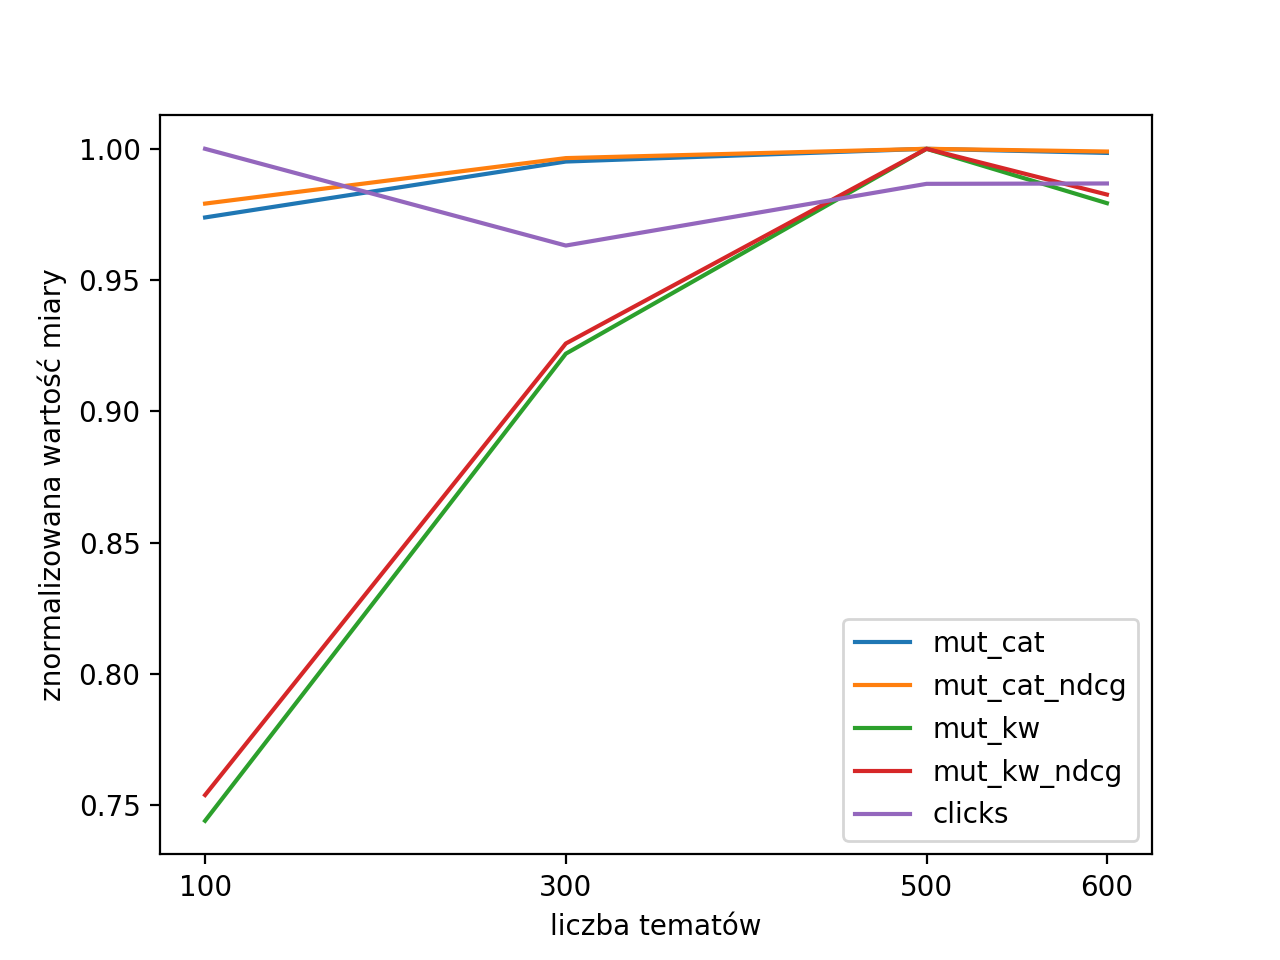
\includegraphics[width=1\textwidth]{img/results/lsi_.png}
		\end{figure}
	\end{frame}
	\begin{frame}{LDA w zależności od liczby tematów}
		\begin{figure}[H]
			\centering
			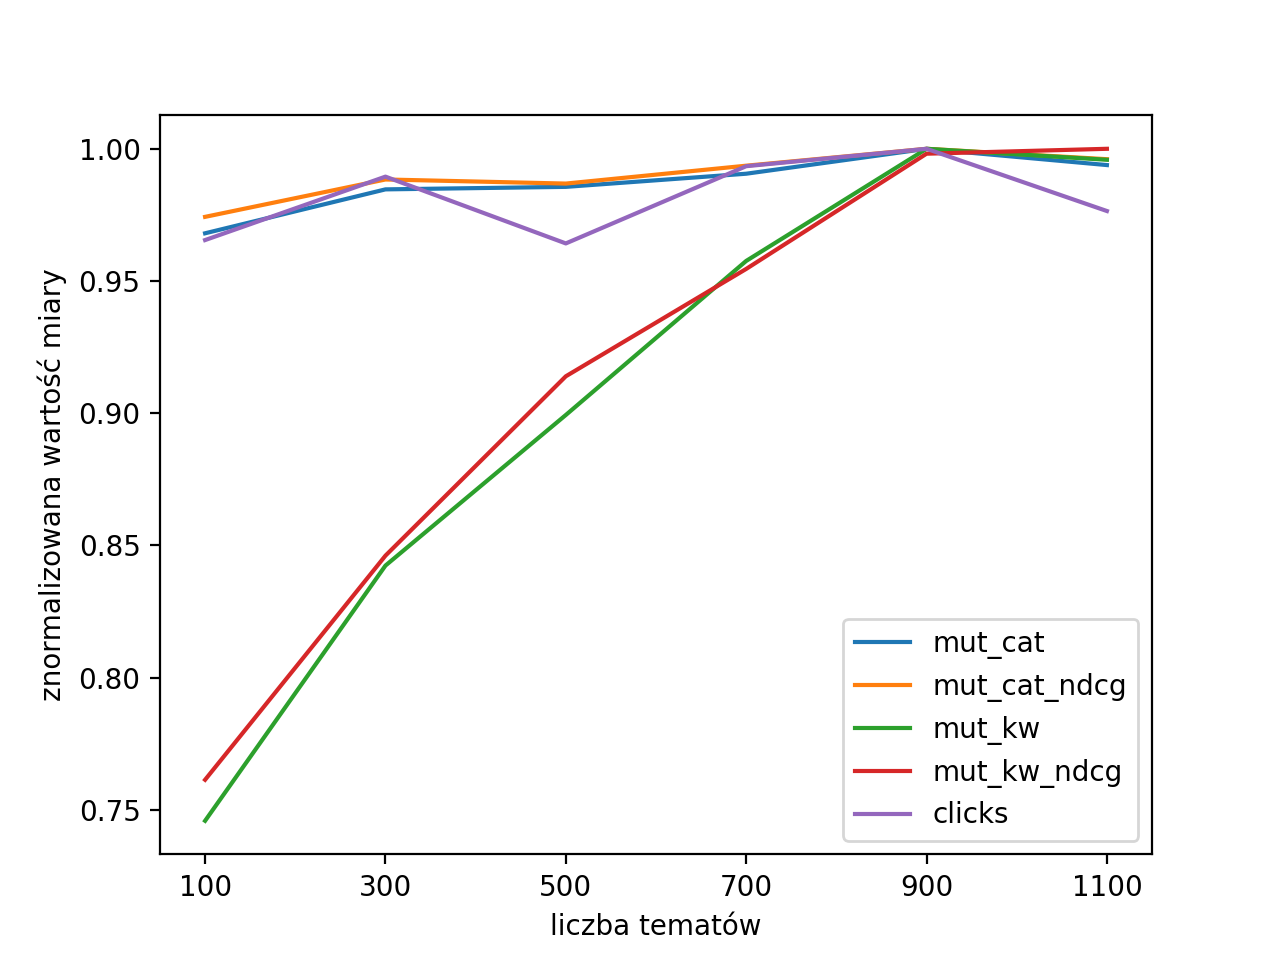
\includegraphics[width=1\textwidth]{img/results/lda_.png}
		\end{figure}
	\end{frame}
	\begin{frame}{Word2vec w zależności od korpusu}
		\begin{figure}[H]
			\centering
			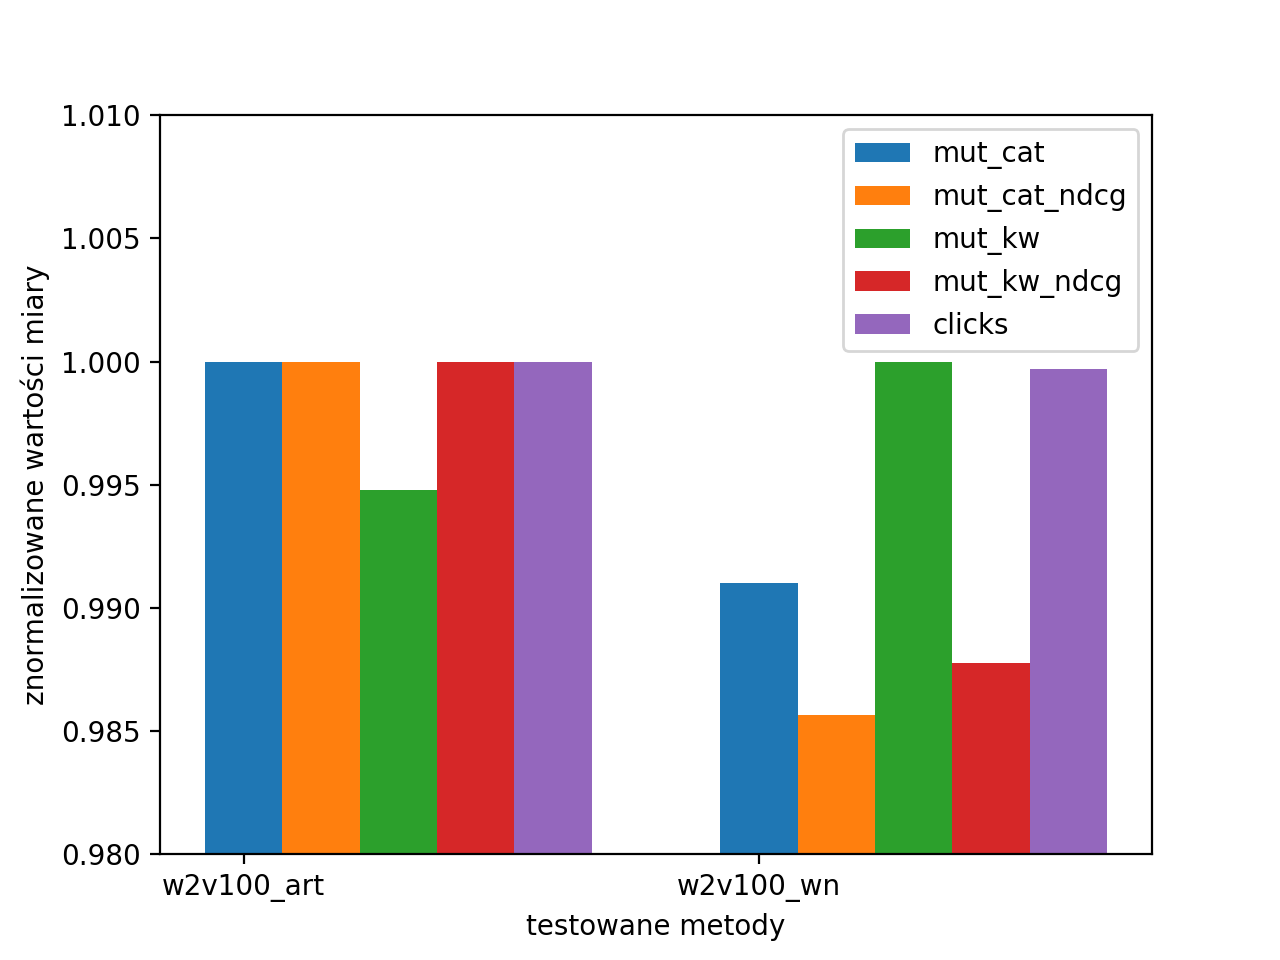
\includegraphics[width=1\textwidth]{img/results/w2v100_art_w2v100_wn_.png}
		\end{figure}
	\end{frame}
	\begin{frame}{Word2vec w zależności od długości wektorów}
		\begin{figure}[H]
			\centering
			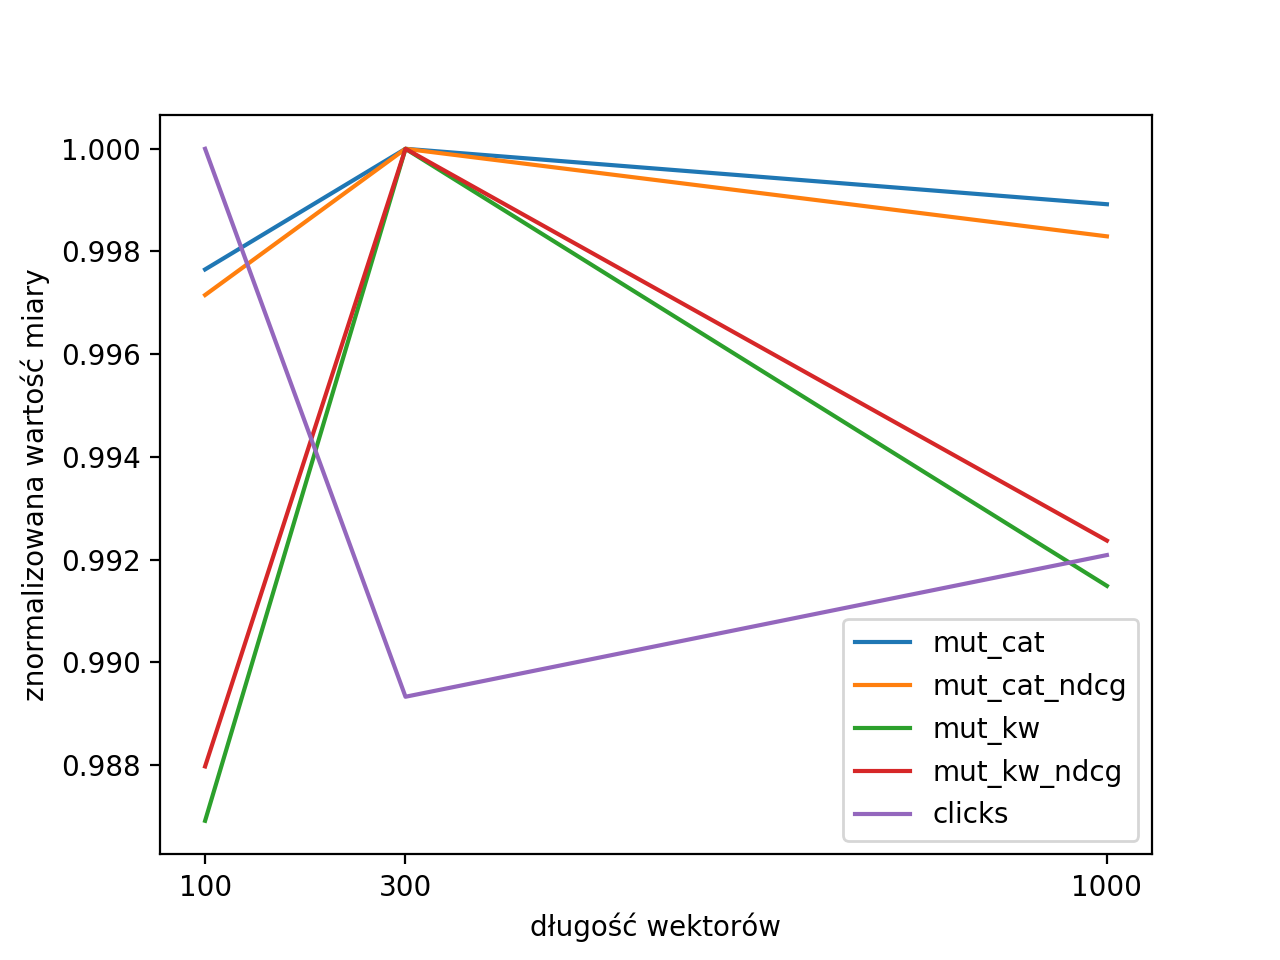
\includegraphics[width=1\textwidth]{img/results/w2v_ctr.png}
		\end{figure}
	\end{frame}
	\begin{frame}{GloVe w zależności od długości wektorów}
		\begin{figure}[H]
			\centering
			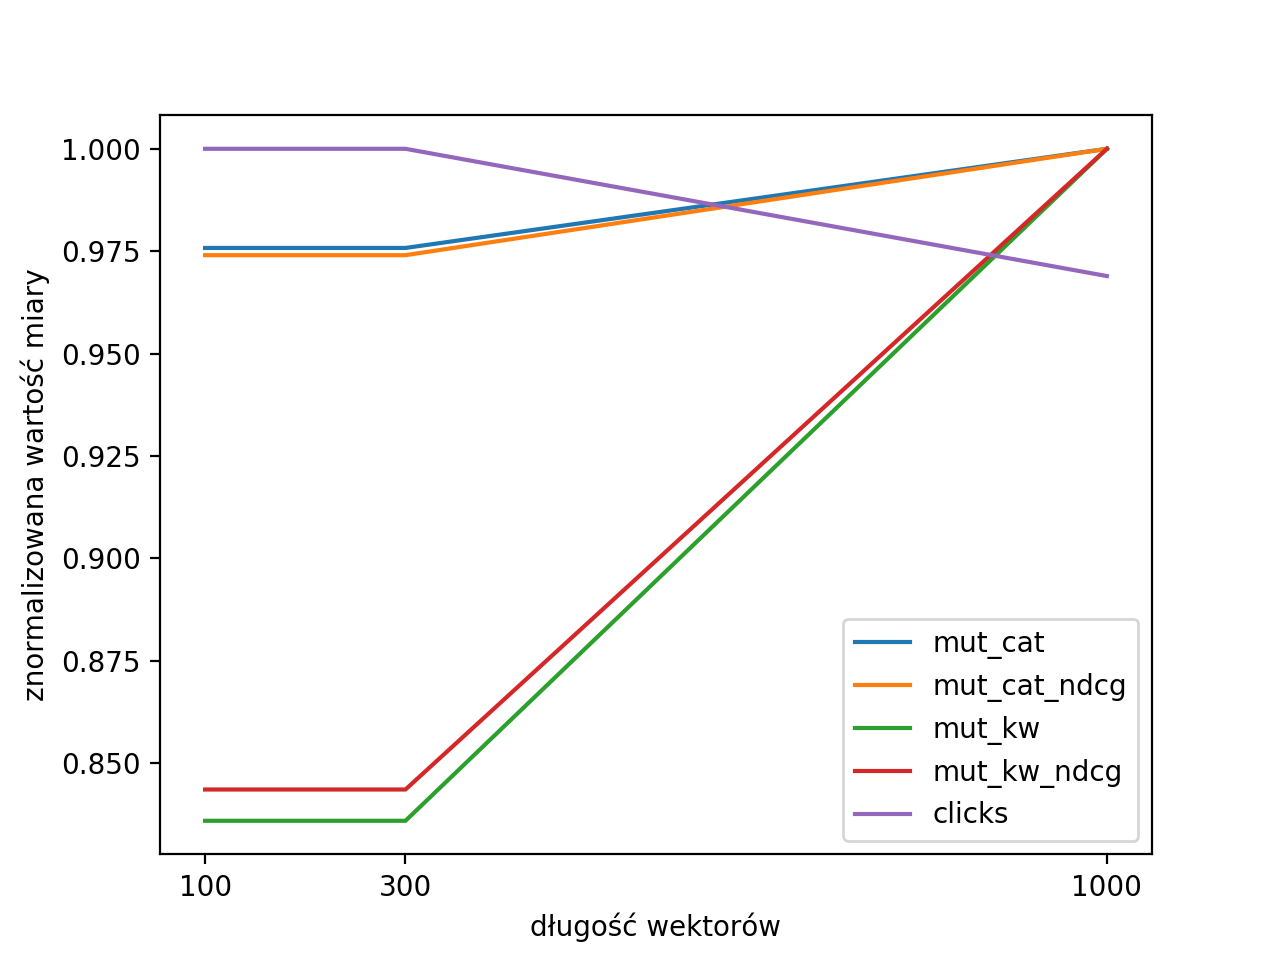
\includegraphics[width=1\textwidth]{img/results/gv_ctr.png}
		\end{figure}
	\end{frame}
	\begin{frame}{FastText w zależności od długości wektorów}
		\begin{figure}[H]
			\centering
			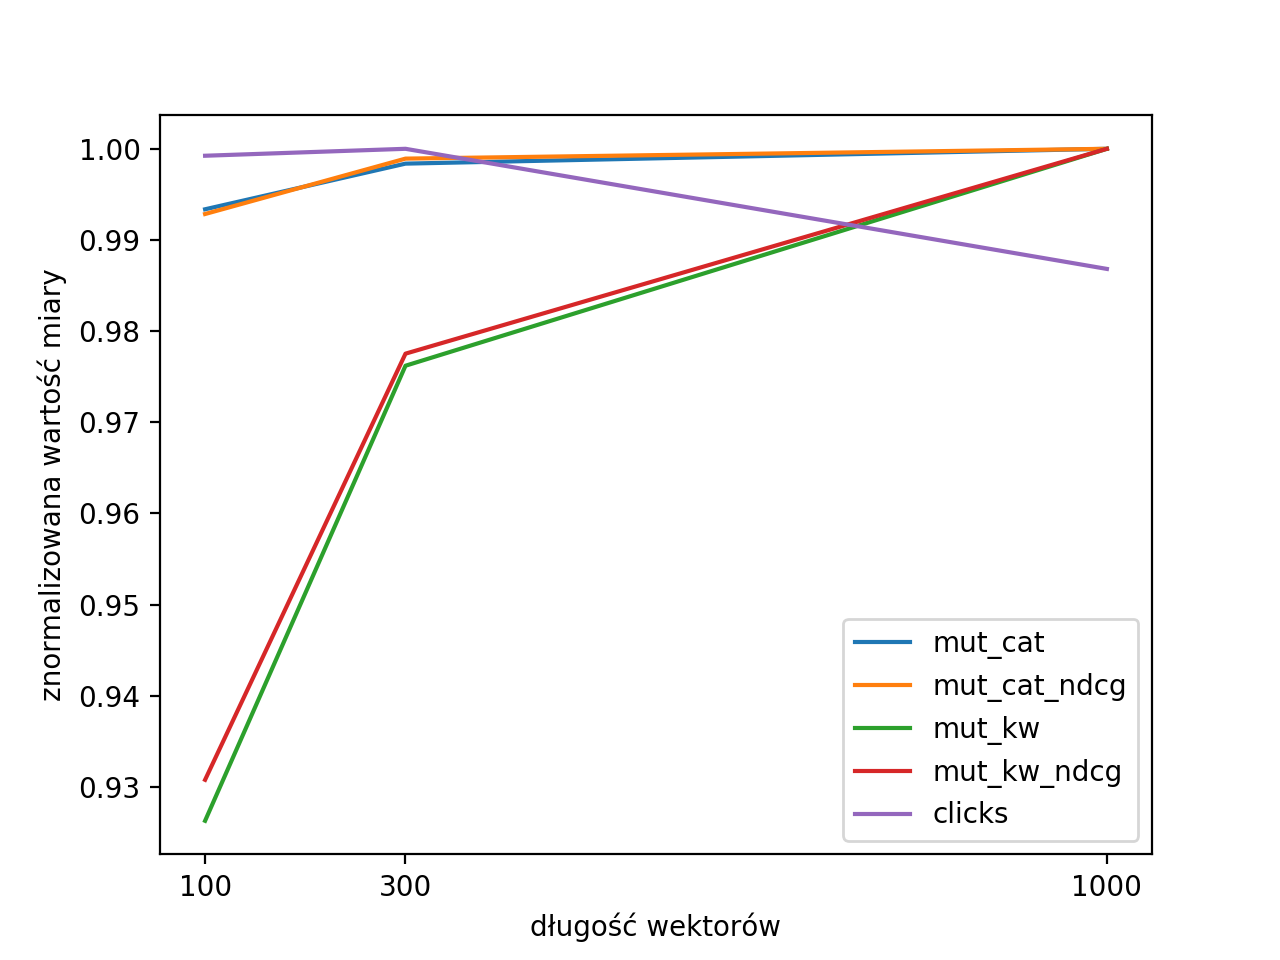
\includegraphics[width=1\textwidth]{img/results/ft_ctr.png}
		\end{figure}
	\end{frame}
	\begin{frame}{Wyniki ewaluacji eksperckiej dla~wybranych metod}
		\begin{figure}[H]
			\centering
			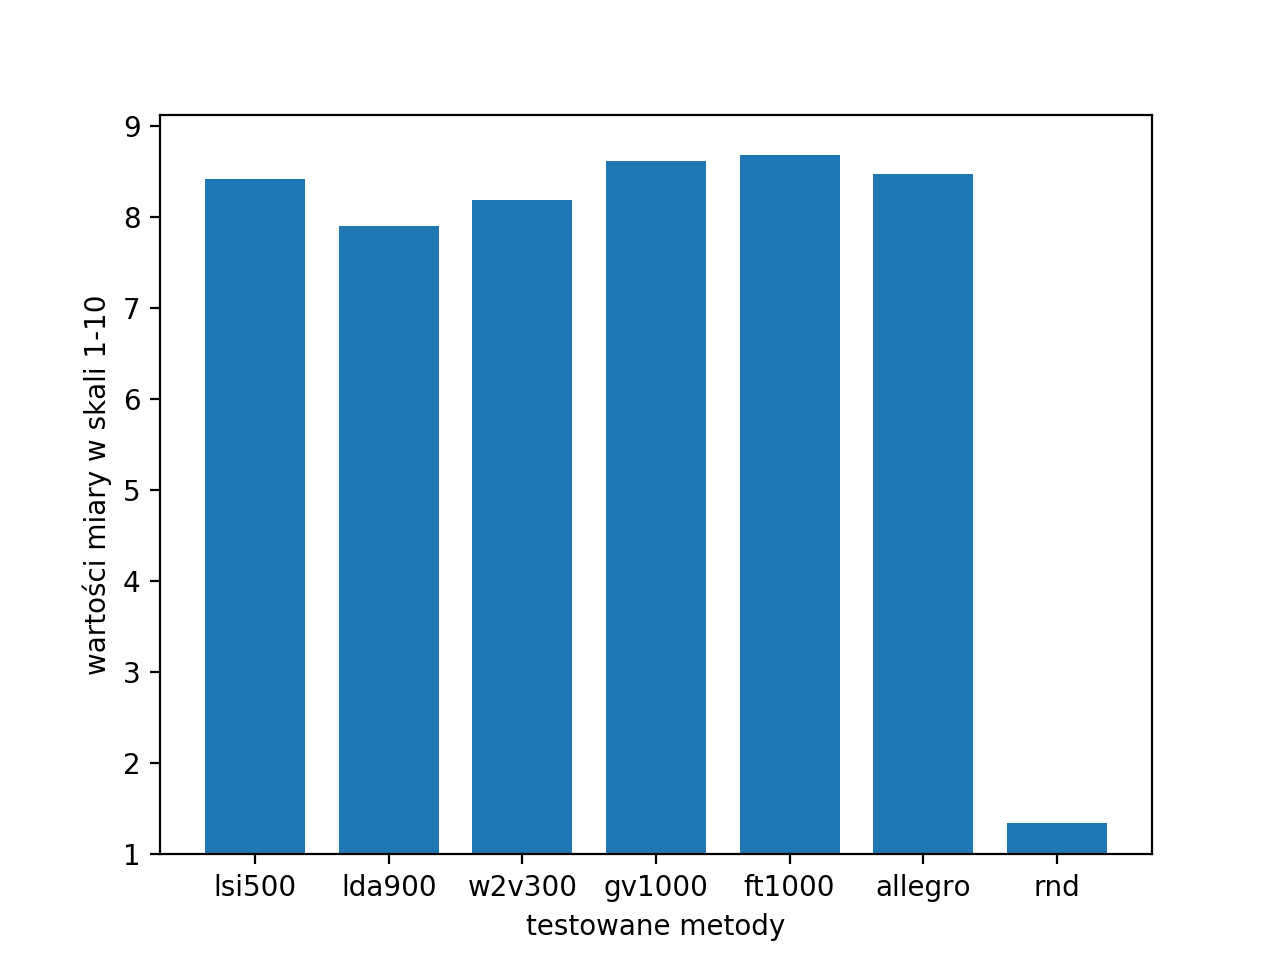
\includegraphics[width=0.8\textwidth]{img/results/lsi500_lda900_w2v300_gv1000_ft1000_allegro_rnd_users.png}
		\end{figure}
	\end{frame}
	\begin{frame}{Porównanie odchyleń standardowych ocen eksperckich dla~wybranych metod}
		\begin{figure}[H]
			\centering
			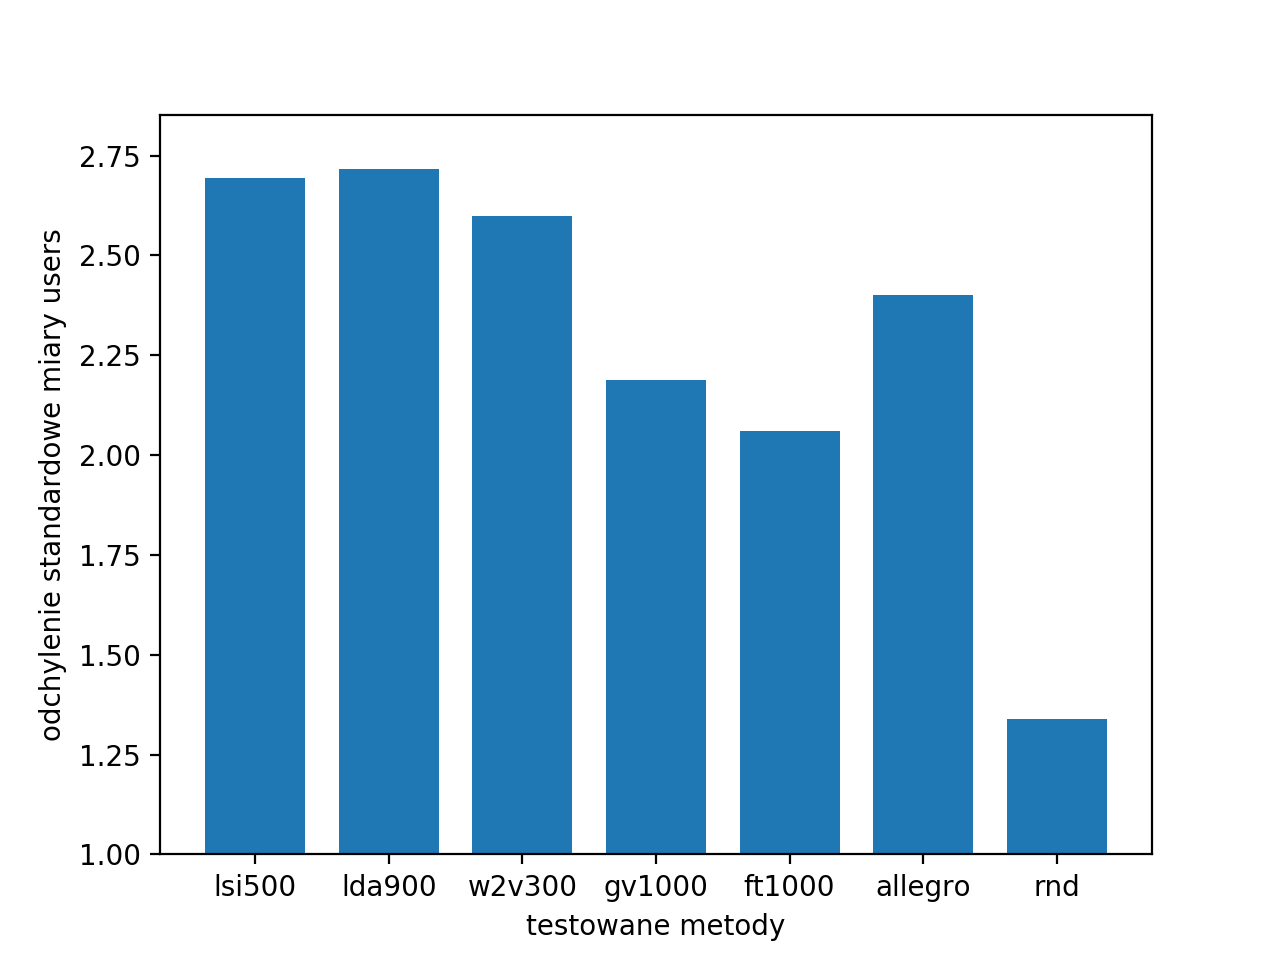
\includegraphics[width=0.8\textwidth]{img/results/lsi500_lda900_w2v300_gv1000_ft1000_allegro_rnd_users_std.png}
		\end{figure}
	\end{frame}
	\section{Podsumowanie}
	\begin{frame}{Podsumowanie testów}
		\begin{itemize}
			\item Brak istotnych statystycznie różnic między wynikami wszystkich metod \pause
			\item Im dłuższe wektory \emph{word embeddings} tym lepsze rezultaty \pause
			\item Większa liczba tematów nie implikuje lepszych rezultatów \pause
			\item ...
		\end{itemize}
	\end{frame}
	\begin{frame}{Kiernki dalszych badań}
		
	\end{frame}
	\begin{frame}{Wnioski}
		testowane metody nie odbiegają jakością od dotychczasowej.
		python
		elasticsearch
		nlp
		trudno jest zmierzyc efekty
	\end{frame}
	\section{Wybrane źródła}
	\begin{frame}{Wybrane źródła}
		content...
	\end{frame}
\end{document}
